\section{Trade-offs} \label{sec:trade-offs}
\subsection{Circuit overhead}
Let $p$ be the probability that Tor Browser submits an SFO to a sampled CTR on a
fresh independent circuit, and $\mathcal{D}$ a distribution that describes how
many SFOs are presented on a website visit.  As shown in
Equation~\ref{eq:sub-oh}, we can now estimate the resulting circuit overhead.
\begin{equation} \label{eq:sub-oh}
	f(p,\mathcal{D}) =
		\frac{p}{n} \sum_{i=1}^{n} c_i, \textrm{where } c_i\sample\mathcal{D}
\end{equation}

We decided to approximate $\mathcal{D}$ using the $n$ most popular webpages
submitted to Reddit (r/frontpage, all time) as of December 4, 2019.\footnote{%
	\url{https://github.com/pylls/padding-machines-for-tor/commit/353bfa75e9f7d6aa0a1dff9516ff234cbf0f4562}
} This was motivated by the intuition that such webpages should include more
resources than basic frontpages, such that $\mathcal{D}$ is more likely to be
overestimated rather than underestimated.  This should further be the case
because we collected the SFO data set using fresh Chromium instances, simply
harvesting all SFOs that appeared in NetLog.  In other words, due to some
initial call-home behavior on start-up, a few additional SFOs are included per
data point.

Using $p=\frac{1}{10}$ and plugging our approximated $\mathcal{D}$ into
Equation~\ref{eq:sub-oh}, the resulting circuit overhead is $0.70$.  It should be
noted that these circuits are \emph{light} in terms of bandwidth when compared
to loading an entire website.

\begin{figure}
	\centering
	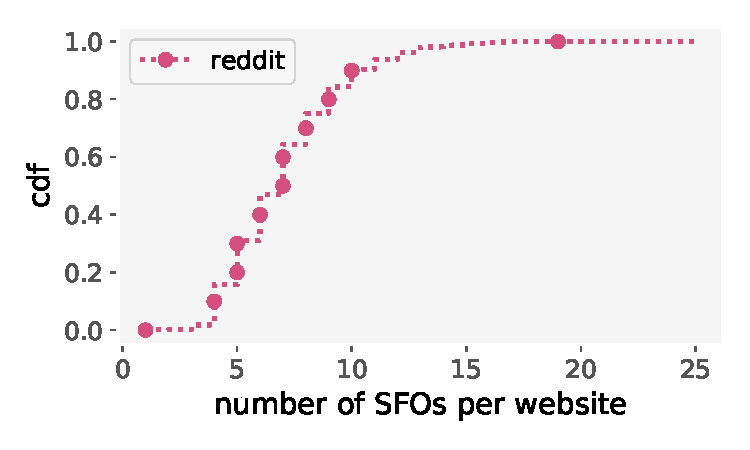
\includegraphics[width=\columnwidth]{../exp/plot/img/sfo-dist}
	\caption{%
		SFO distribution derived from the most frequently viewed reddit pages as
		of December 4, 2019.
	}
	\label{fig:sfo-dist}
\end{figure}

\subsection{SFO Timeouts}
Large timeouts imply less chance that an SFO is leaked to more parties
unnecessarily (privacy).  Small timeouts reduce the attacker's window to
intervene (security).

\subsubsection{Tor Browser}
Recommend a value based on transmitting \texttt{ct-max-sfo-bytes} over many
independent circuits, which gives us a distribution that can be considered.

\subsubsection{CTR}
%Recommend a value based on fetching inclusion proofs from several different
%logs over Tor, which gives us a distribution that can be considered.  Use the
%results from Tor Browser and CTR to reason about \texttt{ct-report-timeout}.

To recommend a timeout value that CTRs could use while challenging the logs to
prove inclusion, we timed how long it takes to fetch inclusion proofs over
Tor from four independent CT logs:
	DigiCert's Log Server~2,
	Sectigo's Sabre,
	Cloudflare's Nimbus 2019, and
	Google's Argon 2019.
The data set was collected using \texttt{torify} and ten SCTs from Alexa's
top-sites, selecting a new circuit after failure (including a warm-up query
to test that the log is responsive) or at most ten subsequent successful
inclusion proofs.  The latter ensures that our data set represents a diverse set
of Tor circuits, as we collected $122$k data points per log in November 2019.

During our measurements we concluded that a query failed if the log 
provided no inclusion proof within ten seconds.  While plotting the results,
we enforced a three-second timeout because it had minimal impact on the final
success rate:
	$0.998$ for the least responsive log (Nimbus), and
	$0.999$ for the three remaining logs.
As shown in Figure~\ref{fig:incl-dist}, it rarely takes more than $1.5$ seconds
to fetch an inclusion proof over Tor.  By doubling that time, we get a
conservative timeout that avoids premature auditor submissions (less leakage)
while at the same time enforcing a short time window during which the attacker
may intervene with any follow-up auditing.

\begin{figure}
	\centering
	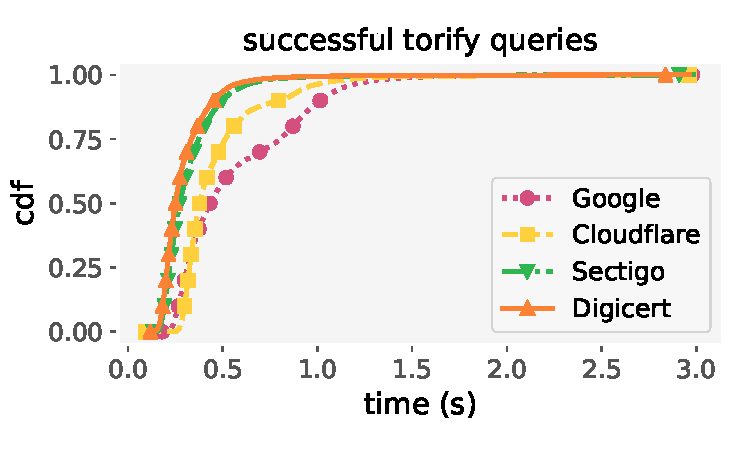
\includegraphics[width=\columnwidth]{../exp/plot/img/incl-dist__torify}
	\caption{%
		Distribution that captures the time it takes to fetch proofs of
		inclusion over already established Tor circuits.  Note that timed-out
		queries are not shown, which ranges from $0.1$--$0.2$\% per log.
	}
	\label{fig:incl-dist}
\end{figure}

\subsection{Flushing}
\label{sec:flooding}

As described in Section~\ref{sec:adversary}, an adversary might attempt to
prevent an offending SFO from being sent to auditors by flooding
one or all CTRs with SFOs. Abstractly, this could have two possible
effects. If CTRs have a limited cache, which, once full, will not
accept new SFOs, then the adversary can block the offending SFO
from ever being held by any CTR by attempting to fill all
CTR caches. If, however, a CTR might drop some cached SFOs
so as to be able to cache some or all newly received SFOs, then
the adversary can try to flush the cache of any CTR that might
hold the offending SFO by flooding that CTR with new SFOs.

A flooding attack could be directed at specific CTRs
known or suspected of holding or being the intended recipient of
an offending SFO\@. Our design, however, limits the ability of
an adversary to know in advance the CTR to which a client will
submit an offending SFO, or to know which CTR is holding
an offending SFO until the CTR sends it to a log for auditing.
And, at that point, there is no longer any point in flushing
or blocking the CTR's cache.

To have sufficient chance of succeeding, flooding attacks must thus be
conducted against all CTRs in the network. To block, this would need to
be sustained in anticipation of an offending SFO being received by
a client or spun up quickly enough after a connection on which an
offending SFO will be sent is initiated to fill all caches within
seconds. Either would be highly visible and would require a
DoS of Tor network resources that exceeds our threat model.\\
***Need to justify that.***

A flushing attack on all CTRs in the network has different time and
knowledge parameters. The adversary need not flush CTRs before an
offending SFO is sent. Indeed, that would be pointless. Once sent,
however, the adversary must sustain a flooding attack so that the
probability that the offending SFO is in any cache at the time of
audit is very low. This gives the adversary effectively an interval
of at least MMD to flush all CTR caches.

To counter flushing, a CTR might adopt a combined strategy of caching
some SFOs with a fixed or parameterized probability and dropping some
SFOs from the cache with a separate fixed or parameterized
probability. To simplify both design and analysis, our CTRs accept all
inbound SFOs. Even if this exceeds the capacity of the cache, we
assume the adversary is not able to exceed the combined capacity of
the cache and inbound buffer. All cached and recently received SFOs
are thus pooled together when considering which to drop. 

By submitting an SFO for auditing at the earliest opportunity a CTR
minimizes the risk of it being flushed and the load on its cache. On
the other hand, by expanding the range of the random delay a CTR adds
to MMD before auditing we expand the uncertainty of the adversary
about whether or not the SFO might still be submitted, thus requiring
him to both spend more resources and increase the risk of exposure by
sustaining the flooding attack for a longer period.

Overhead of a flushing attack for the adversary could be significantly
raised and probability of attack success significantly diminished by
following a strategy used by some types of mix in anonymous
communication: make probabilistic the selection of individual SFOs
amongst both the cached and newly received SFOs to be dropped as
capacity of the cache is exceeded~\cite{trickle02}.


Parameters:

total CTR SFOs: those in the cache plus those in the inbound buffer\\
CTR cache size\\
randomized delay, uniform or decaying distribution?\\

dropping strategies:

uniform = total/cache-size\\
MMD parameterized: Drop SFOs < MMD with one (lower) distribution,
SFOs $\geq$ MMD with another (higher)\\
Dynamic MMD parameterized: Drop only SFOs past MMD + constant until
SFOs not yet to MMD exceeds cache size (following a Poisson or
binomial distribution) . If only SFOs not yet to MMD are in the cache,
then drop SFOs with a distribution that makes it more likely
to drop a newer SFO from the cache until there are again some
above MMD + constant.

Advantage of the latter, is that it requires more resources for
preventing an SFO from even making it to MMD. And by having randomized
delays that follow, e.g., a Poisson or binomial distribution,
the expected time an SFO must be cached is diminished and the
chance of auditing before a flush is increased, even if
the adversary optimizes its flooding strategy.




%%% Local Variables: 
%%% mode: latex 
%%% TeX-master: "../main"
%%% End:          
